%\documentclass[a4paper,justified]{tufte-book}
\chapter{Diffraction} %% created by Martin Braquet

La largeur des fentes n'est pas prise en compte dans le chapitre précédent et conduit à une approximation du phénomène physique. Une fente de largeur finie ne peut pas se représenter comme une unique source d'ondes. La \textit{diffraction} est le comportement non idéal des ondes lorsqu’elles rencontrent un obstacle ou une ouverture.

\begin{figure}[h]
    \centering
    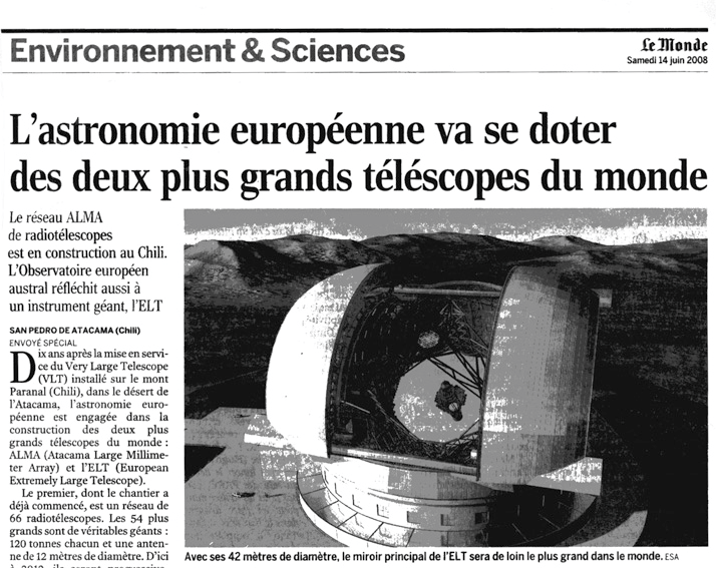
\includegraphics[scale=0.4]{M20}
    \caption{Projet de construction de deux télescopes européens}
    \label{tele}
\end{figure}

\noindent Les 4 télescopes optiques (voir fig \ref{tele})
nommés \textit{VLT} (européens) implantés au Chili ont chacun un diamètre de 8,2 m.
L'amélioration de la précision des télescopes nécessite d'augmenter leur diamètre. La diffraction explique ce constat le long de ce chapitre.

\section{Diffraction par une fente de petite taille}

On considère un rayon lumineux dirigé vers une plaque opaque percée d'une fente de forme rectangulaire d'une largeur de l'ordre du micromètre. Le rayon est dévié dans toutes les directions qui sont dans le demi-cercle opposé à l'apparition du rayon. On remarque sur la figure \ref{d1} que l'intensité dépend de l'angle $\theta$ de la déviation du rayon par rapport à la direction initiale du rayon incident. Contrairement au chapitre précédent, l'intensité est nulle lorsque $\theta$ tend vers $\pm \pi/2$, ce constat est en accord avec les expériences réalisées au cours.

\begin{figure}[h]
    \centering
    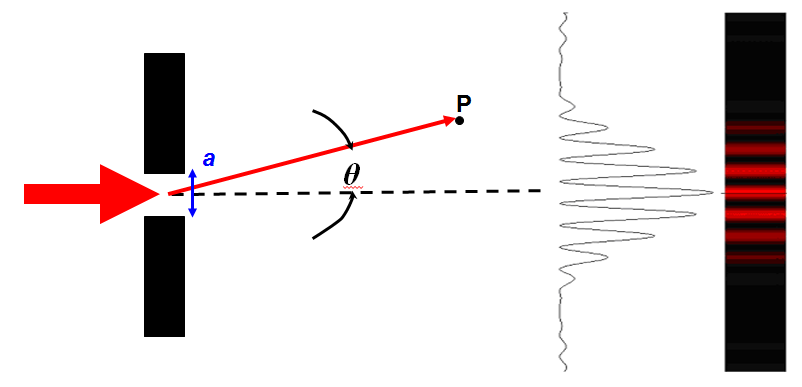
\includegraphics[scale=0.5]{M21}
    \caption{Diffraction par une fente de petite taille}
    \label{d1}
\end{figure}


\noindent Par le principe de Huygens, l'onde traversant cette petite fente peut être remplacée par un ensemble de toutes petites sources les unes à côté des autres et rayonnant dans toutes les directions. Supposons que l'on a $N$ petites sources séparées d'une distance $d$ couvrant la largeur $a=Nd$ de la fente.

\begin{figure}[h]
    \centering
    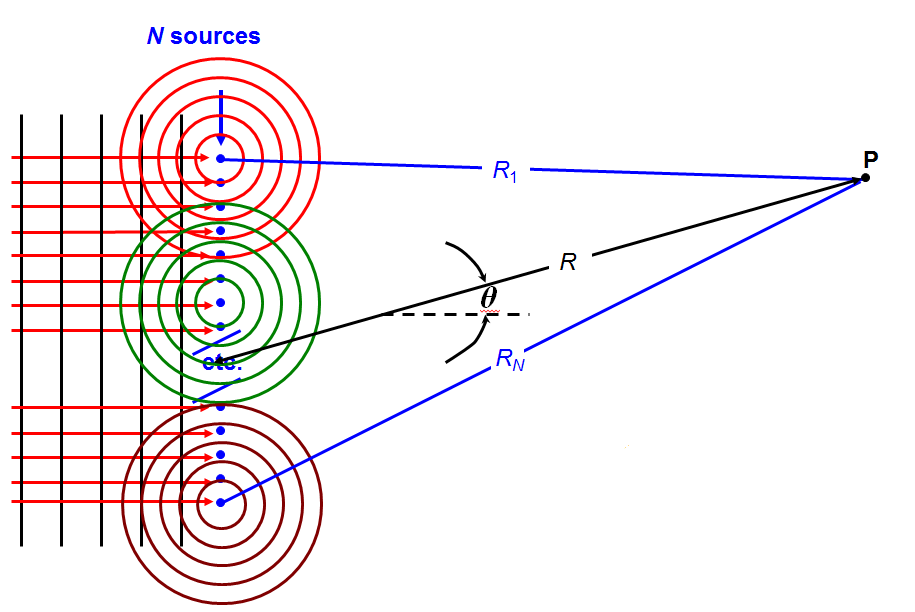
\includegraphics[scale=0.6]{M23}
    \caption{Diffraction par une fente de petite taille, représentée par $N$ sources}
    \label{f2}
\end{figure}

\noindent Sur la figure \ref{f2}, on calcule l'intensité en $P$ résultant de la somme des ondelettes. Le problème est formellement identique à celui traité pour le cas de N fentes idéales.

\noindent Néanmoins, en réalité le nombre de sources $N$ n'est pas fini. On adapte donc la formule de l'intensité pour un réseau de fentes du chapitre sur les interférences en faisant tendre vers $0$ la distance $d$ entre les sources tout en gardant la largeur de le fente $a=dN$ constante. Puisque le nombre de sources est augmenté, il convient de diminuer l'amplitude de chacune de ces sources de manière à conserver la somme des amplitudes: $A \rightarrow A/N=Ad/a$.

\begin{align*}
I(P) & =I_0\lim_{d\to 0} \frac{d^2}{a^2}\frac{\sin^2(\frac{Nd\pi \sin\theta}{\lambda})}{\sin^2(\frac{\pi d\sin\theta}{\lambda})}\\
& \overset{\frac{0}{0}}{=} I_0\lim_{d\to 0} \frac{\sin^2(\frac{a\pi \sin\theta}{\lambda})}{a^2}\frac{2d}{2\sin(\frac{d\pi \sin\theta}{\lambda})\cos(\frac{d\pi \sin\theta}{\lambda})\frac{\pi \sin\theta}{\lambda}}\\
& =I_0 \lim_{d\to 0} \frac{\sin^2(\frac{a\pi \sin\theta}{\lambda})}{a^2}\frac{2d}{\sin(2\frac{d\pi \sin\theta}{\lambda})\frac{\pi \sin\theta}{\lambda}}\\
& \overset{\frac{0}{0}}{=}I_0 \lim_{d\to 0} \frac{\sin^2(\frac{a\pi \sin\theta}{\lambda})}{a^2}\frac{2}{\cos(2\frac{d\pi \sin\theta}{\lambda})2(\frac{\pi \sin\theta}{\lambda})^2}\\
& =I_0 \frac{\sin^2(\frac{\pi a \sin\theta}{\lambda})}{(\frac{\pi a \sin\theta}{\lambda})^2}.
\end{align*}

\begin{figure}[h]
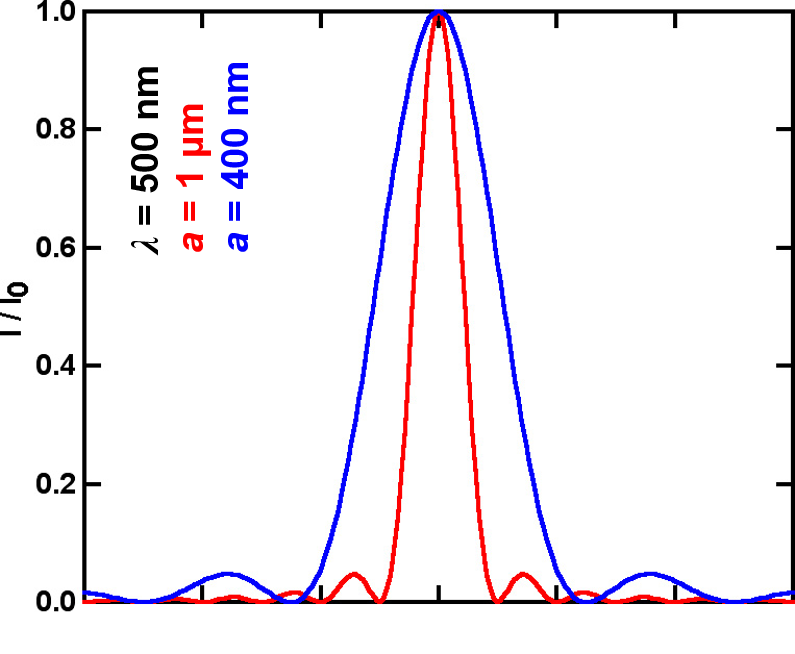
\includegraphics[scale=0.6]{M25}
\caption{Intensité d'un rayon lumineux traversant une fente}
\label{f3}
\end{figure}

\noindent Cette équation montre qu'une grande fente génère des lobes plus étroit. L'intensité, présentée sur la figure \ref{f3}, s'annule lorsque
$$
  \frac{\pi a \sin\theta}{\lambda}=m\pi \Rightarrow a \sin\theta = m\lambda \qquad(\forall m\in  \mathbb{Z}_0).
$$

\noindent Cette relation permet donc de mesurer la largeur d'une fente (ou on le verra plus tard, d'un objet). En mesurant expérimentalement l'angle donnant lieu au premier lobe, $a$ peut être déterminé.\\

\noindent On pourrait également vouloir calculer les positions des maxima locaux d'intensité. Contrairement à ce qu'une observation rapide de l'équation ci-dessus pourrait laisser penser, les pics ne se produisent pas exactement quand la fonction sinus vaut $\pm1$. La dérivée de l'intensité par rapport à $\theta$ est une équation transcendante qui s'annule à des positions correspondant à un maximum pour 
\[
\frac{2\pi}{\lambda}a \sin\theta\simeq
\left\{
\begin{array}{c}
 2,86\pi\\
 4,92\pi    \\
...
\end{array}
\right.
\Longrightarrow
I\simeq
\left\{
\begin{array}{c}
 0,0472I_0 \mbox{ (1er pic)}\\
 0,0165I_0 \mbox{ (2e pic)}\\   
  ...
\end{array}
\right.
\]
Ces intensité diminuent très rapidement, le premier pic valant seulement $5\%$ du pic central. Dans les chapitres suivants, on approximera donc parfois la figure de diffraction par un unique lobe.

\section{Diffraction par un objet de petite taille}

Il est possible de montrer que la lumière est diffractée de la même façon en traversant une fente ou un objet de même taille. Pour prouver cela, on considère d'abord, selon le principe de Huygens, et pour une onde se propageant dans le vide (sans obstacle), la représentation d'un front d'onde par une multitude de petites sources (fig \ref{f4}). Le champ généré plus loin dans la direction de propagation de l'onde (ici vers la droite) est obtenu par la somme des ondelettes créées par chacune des petites source (les cercles turquoises sur la figure). On le dénote par $\overset\rightarrow{E}_0$.

\begin{marginfigure}[0cm]
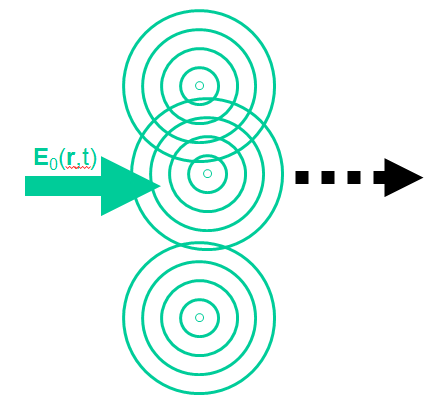
\includegraphics[width=1\textwidth]{M26}
\caption{Représentation d'un front d'onde par une multitude de sources}
\label{f4}
\end{marginfigure}

\noindent Pour analyser les effets de diffraction d'une fente et d'un objet, on décompose ensuite ce front d'onde en deux parties (fig \ref{d2}):
\begin{itemize}
    \item l'ensemble des sources bleues se trouvant en dehors d'un petit objet de largeur $a$ et dont la somme des ondelettes transmises correspond à l'effet de diffraction par cet objet. On dénote l'onde correspondante par $\overset\rightarrow{E}_2$
    \item l'ensemble des sources rouges se trouvant à l'intérieur de la fente de largeur $a$ et dont la somme des ondelettes transmises correspond à la diffraction par cette fente. On dénote l'onde correspondante par $\overset\rightarrow{E}_1$
\end{itemize}

\begin{figure}[h]
    \centering
    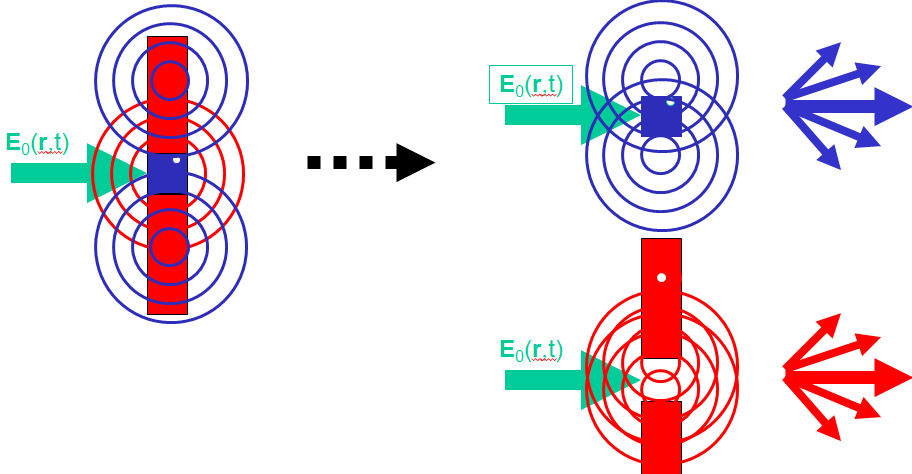
\includegraphics[scale=0.4]{M27}
    \caption{Diffraction par une fente ou un objet}
    \label{d2}
\end{figure}

\noindent Par superposition, il est clair que $\overset\rightarrow{E}_1+\overset\rightarrow{E}_2=\overset\rightarrow{E}_0$. La somme correspond au champ obtenu sans obstacle. Le champ transmis $\overset\rightarrow{E}_2$ correspond au champ créé par la diffraction à travers un objet de largeur $a$ et le champ transmis $\overset\rightarrow{E}_1$ correspond au champ créé par la diffraction à travers une fente de largeur $a$ (établi au paragraphe précédent).
Si on se place en un point $P$ pour lequel $\overset\rightarrow{E}_0(P)=\overset\rightarrow{0}$, on trouve $\overset\rightarrow{E}_1(P)=-\overset\rightarrow{E}_2(P)$, et l'intensité transmise par la fente $I_1\propto |\overset\rightarrow{E}_1|^2$ est égale à l'intensité transmise par l'objet $I_2\propto |\overset\rightarrow{E}_2|^2$. Le principe de Babinet énonce de manière analogue que deux figures de diffraction identiques sont créées lors d'une diffraction par un objet ou une fente de même taille. Ainsi, tout problème de diffraction impliquant une ouverture peut être remplacé par un problème équivalent impliquant un petit objet. Puisqu'il n'y a pas de diffraction si le rayon rencontre une plaque opaque ou s'il n'y a pas d'objet, ce sont les bords qui produisent le phénomène de diffraction.\\

\noindent A titre d'exemple, dans le cas de la diffraction par un cheveu, on observe toujours bien l'impact du laser sur l'écran (correspondant au $\overset\rightarrow{E}_0$), auquel vient se soustraire la figure de diffraction correspondant à une fente. Il s'agit d'une soustraction en terme de champ électromagnétique. Dans toutes les zones en dehors du point d'impact du laser, on observe exactement la même intensité que pour la diffraction par une fente.\\


\begin{marginfigure}[2cm]
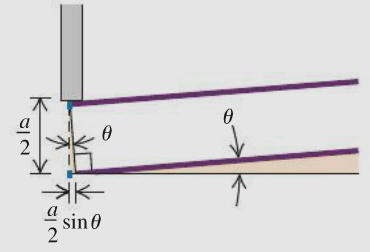
\includegraphics[width=0.9\textwidth]{M55}
\caption{Diffraction par une fente}
\label{f5}
\end{marginfigure}

\noindent Il est possible d'obtenir les directions des franges noires par un raisonnement basé sur l'interférence destructive des ondes créées par une fente de largeur $a$. La différence de chemin (fig \ref{f5}) entre l'onde émise au centre de la fente et celle émise juste en dessous du bord supérieur vaut $a/2\:\sin\theta$. Pour qu'il y ait une interférence destructive, cette distance doit valoir $(2m+1)\lambda/2$. De manière similaire, les deux faisceaux venant de deux sources, décalées d'une distance infinitésimale par rapport aux deux sources précédentes, ont la même différence de chemin et se détruisent aussi. Donc, la lumière de chaque source sur la moitié supérieure de la fente s'annule avec la source correspondante dans la moitié inférieure, donnant ainsi une frange sombre dans cette direction $\theta$. Donc $\sin\theta=\pm\lambda/a$, le signe $\pm$ indique que la figure de diffraction est symétrique. La frange en $\theta>0$ apparaît en $P$ quand la lumière de la moitié inférieure de la fente fait une distance plus grande de $\lambda/2$ que celle de la moitié supérieure. La frange en $\theta<0$ apparaît en $P$ quand la lumière de la moitié supérieure de la fente fait une distance plus grande de $\lambda/2$ que celle de la moitié inférieure. En divisant la fente non plus en 2 mais en 4,6,8, et ainsi de suite, on utilise l'argument ci-dessus pour montrer qu'une interférence destructive se produit quand $\sin\theta=\pm\lambda/a,\pm2\lambda/a,\pm3\lambda/a,\pm4\lambda/a$,...
Finalement, on peut reformuler la relation pour obtenir
$$
    \sin\theta=\frac{m\lambda}{a}\qquad(\forall m\in  \mathbb{Z}_0).
$$
qui était déjà établie auparavant.

\section{Pouvoir séparateur d'un instrument d'optique (ou pouvoir de résolution spatiale) }

La diffraction est un des effets principaux limitant la précision des instruments d'observation optiques (ou plus généralement observant des ondes).

\noindent Le microscope optique possède une lentille d'environ 5 mm de diamètre pour observer des objets visibles (correspondant à des longueurs d'onde entre 380 et 780 nm).

\noindent Le radiotélescope d'Arecibo sur la figure \ref{f6} a une parabole d'environ 305 m de diamètre focalisant les ondes électromagnétiques pour observer des objets émettant avec une longueur d'onde de 10 cm. Ce télescope situé à Porto Rico est opéré par l'Université de Cornell.

\begin{marginfigure}[-2cm]
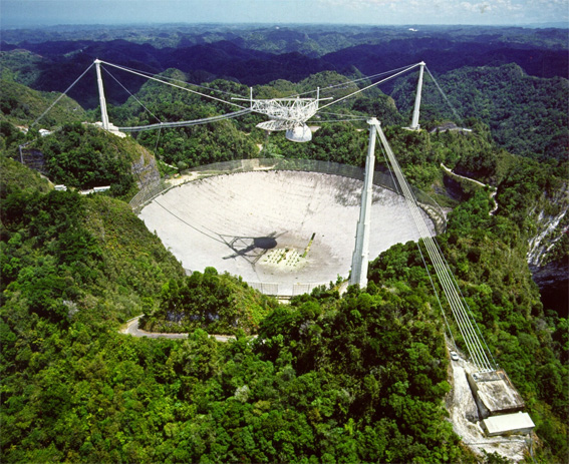
\includegraphics[width=0.9\textwidth]{M29}
\caption{Radiotélescope d'Arecibo}
\label{f6}
\end{marginfigure}

\noindent Le rapport $\lambda/a$ entre la longueur d'onde et la taille de l'ouverture est de l'ordre de $10^{-3}$ dans les deux cas et sa raison est explicitée ci-dessous.\\

\noindent Dans les instruments d'optique, on considère que la lumière entre dans une lentille de diamètre $a$. Le passage dans cette ouverture circulaire génère un effet de diffraction. Son analyse mathématique s'effectue de manière presque similaire à celle d'une fente de largeur $a$. La diffraction par une ouverture circulaire engendre une figure de diffraction (appelée tache d'Airy\footnote{du physicien anglais \textit{George Biddell Airy} (1801-1892)}) formée de cercles concentriques dont l'intensité diminue avec le diamètre du cercle. 

\noindent Lorsque la figure est observée loin du trou diffractant (approximation de Fraunhofer), l'intensité varie en fonction de l'angle $\theta$ entre le point considéré et le centre de la figure comme:
$$
    I(\theta)=I_0\bigg(\frac{2J_1(\frac{\pi a\sin\theta}{\lambda})}{\frac{\pi a\sin\theta}{\lambda}}\bigg)^2
$$
où $J_1$ est la fonction de Bessel du premier ordre, $I_0$ est l'intensité au centre de la figure et $\theta$ est l'angle entre l'axe de révolution et la direction considérée.

\noindent La première annulation de cette fonction se produit lorsque 
$$
    a\sin\theta\simeq1,22\lambda.
$$
Cette relation montre que si le rapport $\lambda/a$ est identique pour deux expériences, la même figure de diffraction sera représentée. Les deux cercles sombres suivants sont situés dans les directions $\theta$ vérifiant les relations $a\sin\theta\simeq2,23\lambda$ et $a\sin\theta\simeq3,24\lambda$.

\noindent L'intensité diminue plus rapidement que dans une fente rectangulaire, le pic d'intensité du premier ordre valant seulement $1,7\%$ de l'intensité au centre de la figure. La plupart ($85\%$) de l'énergie lumineuse est située dans le disque central (disque d'Airy).\\

\noindent Pour analyser le pouvoir de séparation d'un instrument d'observation, on considère deux rayons lumineux traversant un trou dans une boite, leur rayon incident n'est pas perpendiculaire à la face possédant le trou (voir fig \ref{d4}).

\begin{figure}[h]
    \centering
    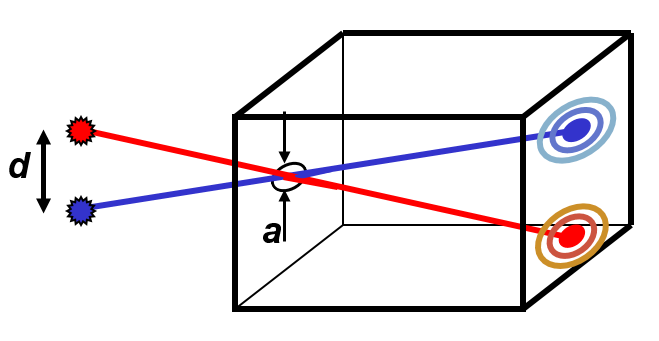
\includegraphics[scale=0.5]{M30}
    \caption{Rayons lumineux traversant un creux dans une boite}
    \label{d4}
\end{figure}

\noindent La figure \ref{d6} illustre la projection des taches de lumière sur la face opposée au creux pour un diamètre $a$ décroissant vers les images de droite.

\begin{figure}[h]
    \centering
    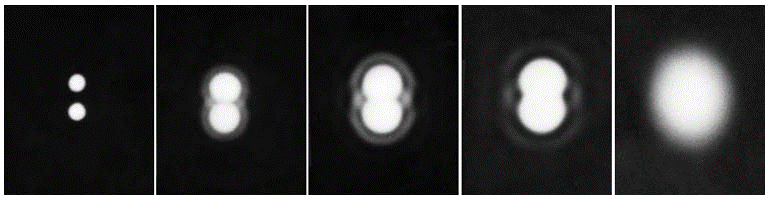
\includegraphics[scale=0.4]{M31}
    \caption{Taches de lumières pour différents diamètres}
    \label{d6}
\end{figure}

\noindent Puisque la largeur des lobes est inversement proportionnelle au diamètre $a$, les taches s'agrandissent avec la diminution du diamètre du creux. Par contre, les taches gardent le même centre car l'angle d'incidence ne change pas.
Les taches deviennent ainsi indissociables en dessous d'une certaine valeur de $a$. \\

\noindent De la même manière, on peut également varier la distance $d$, c'est-à-dire l'angle d'incidence des deux rayons. La figure \ref{d8} présente les taches avec la distance $d$ qui diminue vers les images de droite.

\begin{figure}[h]
    \centering
    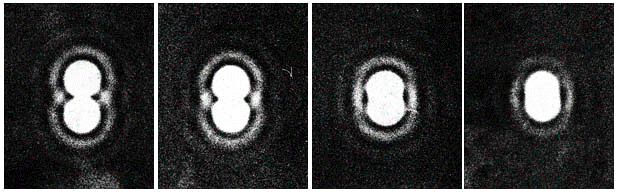
\includegraphics[scale=0.47]{M32}
    \caption{Taches de lumières pour différents angles d'incidence}
    \label{d8}
\end{figure}

\noindent Contrairement à l'expérience précédente, le diamètre des taches, lié à $a$, ne varie pas mais les positions des centres se rapprochent lorsque $d$ diminue. Pour une taille de trou donnée, il y a une distance $d$ (et un angle d'incidence $\theta$) minimum pour laquelle les taches ne se superposent pas. \\

\noindent Pour un œil, il y a aussi l’effet de la lentille qui fait converger les faisceaux vers le même point, excepté les diffractés. Sans cette convergence, il y aurait superposition de la tache qui passe, et des effets de diffraction. Mais la focalisation résultant de la lentille permet de réduire la tache éclairée, et il ne reste plus que l’effet de diffraction.\\

\begin{marginfigure}[0cm]
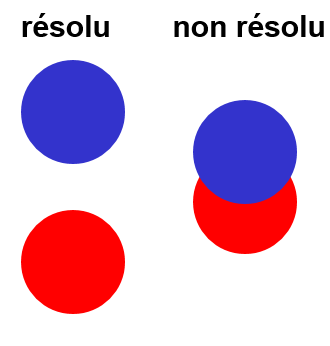
\includegraphics[width=0.9\textwidth]{M33}
\caption{Critère de Rayleigh}
\label{f7}
\end{marginfigure}

\noindent Une relation mathématique peut s'établir en déterminant un critère de résolution (fig \ref{f7}) énoncé par Lord Rayleigh: deux taches sont résolues si le premier lobe de la figure de diffraction d'un des deux faisceaux ne se chevauche pas avec le centre de l'autre rayon lumineux. Cela correspond à la résolution angulaire minimale sous laquelle les deux objets formeront une seule tache. Pour augmenter la résolution en gardant la même distance entre le trou et l'objet ($d$ constant), il faut ainsi augmenter $a$ et/ou diminuer $\lambda$.

\noindent Ainsi, pour discerner les disques lumineux, l'angle d'incidence $\theta_i$ doit être supérieur à l'angle du premier lobe de diffraction $\theta_1$:
$$
    \sin\theta_i>\sin\theta_1
$$
$$
    \sin\theta_i>1,22\lambda/a.
$$
En posant $L$, la distance entre le trou et les deux sources, on peut approximer cette relation pour des petits angles d'incidence tels que $\sin\theta_i=\tan \theta_i$:
$$
    \tan\theta_i=d/L>1,22\lambda/a.
$$

\subsection{Microscopie optique de haute résolution}

\begin{marginfigure}[-1.5cm]
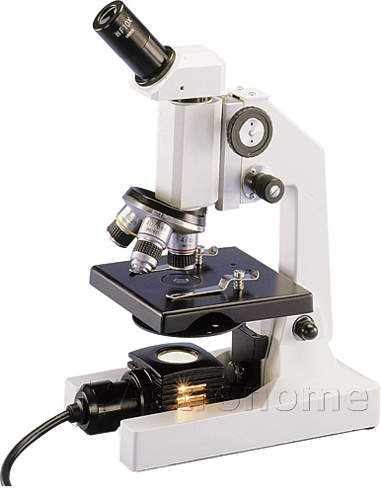
\includegraphics[width=0.9\textwidth]{M34}
\caption{Microscope optique}
\label{f8}
\end{marginfigure}

Les caractéristiques d'un microscope optique (fig \ref{f8}) sont les suivantes: $\lambda\simeq500nm,a\simeq2mm$ et $L\simeq1mm$. La distance de résolution vaut ainsi 
$$
d_{min}=1,22\lambda L/a\simeq300\:nm.
$$
Pour que ce microscope puisse discerner les atomes ($d\simeq0,5nm$), la longueur d'onde devrait être inférieure à $da/(1,22L)\simeq1nm$ (rayons X). Puisqu'il n'existe pas de lentille qui puisse analyser les rayons X, un tel microscope n'est pas assez précis pour voir des atomes.

\subsection{Microscopie électronique de haute résolution}

\begin{marginfigure}[-1cm]
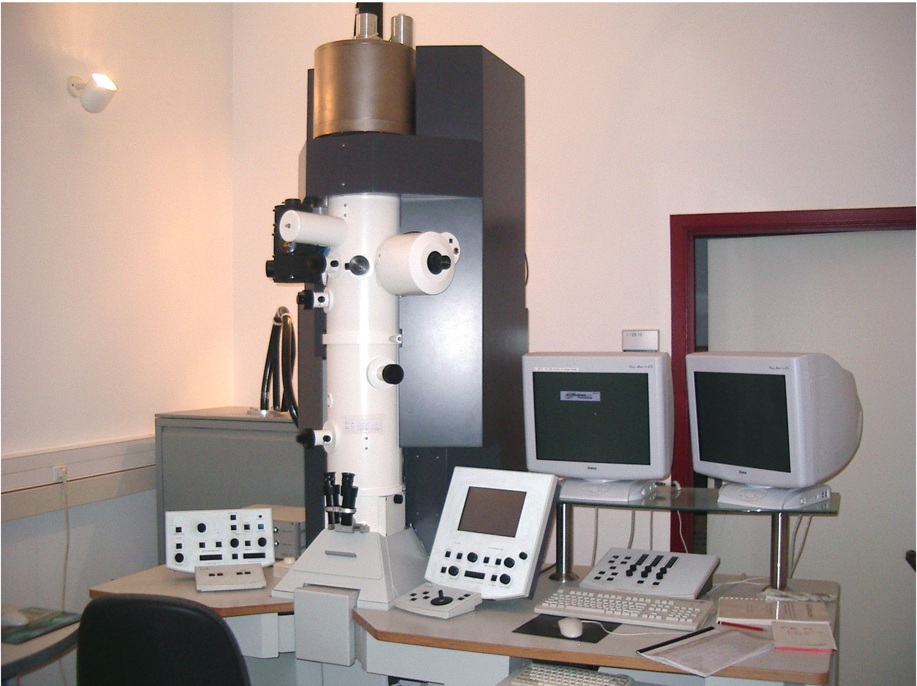
\includegraphics[width=0.9\textwidth]{M35}
\caption{Microscope électronique}
\label{f9}
\end{marginfigure}

Pour améliorer la précision, on peut remplacer les ondes lumineuses par des électrons (fig \ref{f9}), qui ont aussi des propriétés ondulatoires. La longueur d'onde d'un électron est beaucoup plus petite (entre\footnote{cette longueur d'onde dépend de la tension d'accélération des électrons} $0,1$ et $1nm$). Ce dispositif, qui n'exploite plus les ondes visibles, analyse un objet de manière indirecte. Le microscope enregistre ainsi des données électroniques pour les convertir ensuite en une représentation 2D ou 3D. Un microscope électronique à transmission a une résolution de $$d_{min}=1,22\lambda L/a\simeq0,5\:nm$$ puisque $a\simeq L\simeq10mm$.
Néanmoins, il est nettement plus cher et requiert des lentilles magnétiques pour focaliser le faisceau d'électrons.\\

\begin{marginfigure}[0cm]
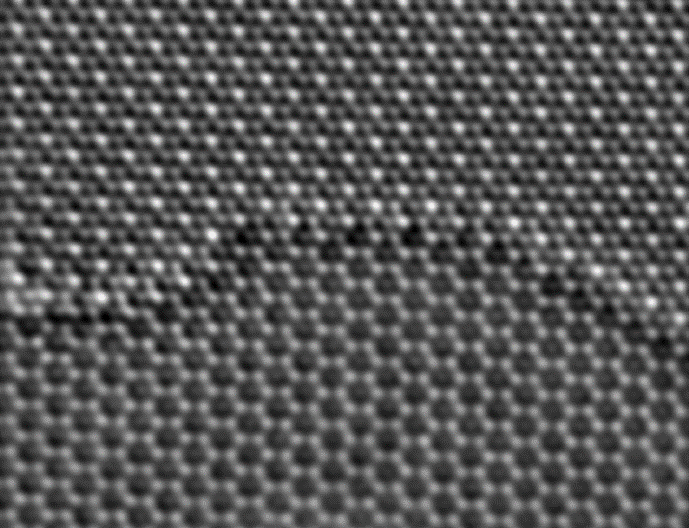
\includegraphics[width=0.9\textwidth]{M36}
\caption{Image d'un échantillon de graphène}
\label{f10}
\end{marginfigure}

\noindent Ce microscope produit par exemple une image précise d'un échantillon de graphène (fig \ref{f10}), un matériau dont la distance interatomique vaut environ $0,15$ nm.\\

\noindent D'autres principes d'imagerie existent également: microscopes à force atomique, microscopes à effet tunnel,...

\subsection{Microlithographie et nanolithographie}

\begin{marginfigure}[0cm]
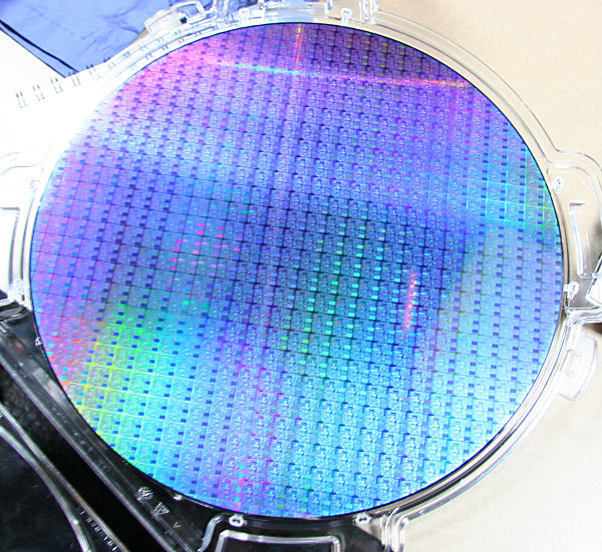
\includegraphics[width=0.9\textwidth]{M37}
\caption{Photolitographie}
\label{f11}
\end{marginfigure}

La microlithographie et la nanolithographie sont deux procédés de fabrication très précise d'objets. Ce système est principalement utilisé pour créer des circuits intégrés dans le domaine de l'électronique. Le substrat est composé d'une couche de polymère photo-sensible (résine) sur un disque en silicium. Pour tracer le circuit, on illumine ce substrat au travers d'un masque réalisé au préalable, ce qui a pour effet de modifier la résine à des endroits précis sur la couche de polymère. Le substrat est ensuite rincé par un solvant sélectif pour enlever les parties du polymère qui ont été exposées aux rayons. On peut ensuite procéder à l'implantation d'ions dans le semiconducteur aux endroits désirés afin de créer le circuit électronique voulu. 

\noindent Le masque en chrome, permettant d'exposer uniquement certaines parties du polymères, agit comme un réseau de fentes et provoque donc la diffraction des ondes. La diffraction limite la précision du circuit car les zones irradiées sur le polymère sont plus grandes que les fentes sur le cache (fig \ref{d9} a). Pour augmenter la densité de transistors par unité de surface,
il faut diminuer l'effet de diffraction, c'est-à-dire l'angle du premier lobe $\theta$. Puisqu'on ne peut pas augmenter la largeur de la fente sans diminuer la précision, il convient d'employer des ondes possédant une longueur d'onde la plus petite possible. La lithographie optique utilise les ondes lumineuses alors que la lithographie électronique (uniquement en laboratoire à l'heure actuelle) utilise des électrons pour leur faible longueur d'onde. La figure \ref{d9} b présente différentes ondes utilisées en correspondance avec leur précision.

\noindent Cette problématique apparaît de façon similaire dans la lecture des CDs et DVDs. Le lecteur optique possède une ouverture (lentille) et est sujet à une certaine diffraction qui limite la précision avec laquelle on peut lire les trous sur le CD. C'est la raison pour laquelle la technologie Blu-ray a évolué vers l'utilisation de lasers de lecture violets (longueur d'onde 400 nm) au lieu de lasers rouges (longueur d'onde 650 nm); ainsi qu'une augmentation de la taille de la lentille.

\begin{figure}[h]
\centering
\subfloat[]{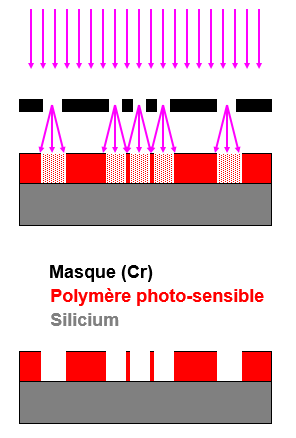
\includegraphics[width=4cm]{M38}}
        \quad
\subfloat[]{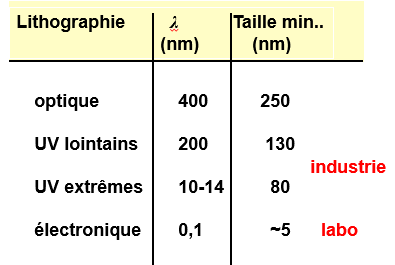
\includegraphics[width=5cm]{M39}}
\caption{Lithographie}
        \label{d9}
\end{figure}

\begin{marginfigure}[0cm]
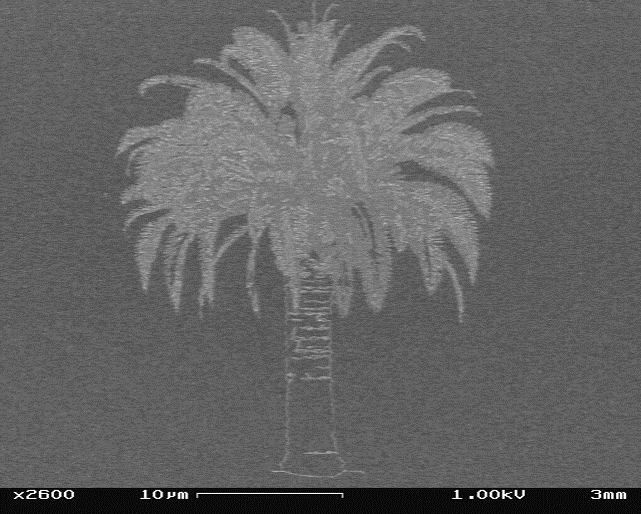
\includegraphics[width=0.9\textwidth]{M40}
\caption{Dessin d'un palmier}
\label{f13}
\end{marginfigure}

\noindent Cette technique est aussi utilisé en science des matériaux pour sculpter très finement la matière. Des chercheurs (fig \ref{f13}) à l'UCL ont par exemple créé le dessin d'un palmier très précis sur une plaque de $50\:\mu m$ de coté.

\section{Réseaux de fentes}

\begin{marginfigure}[0cm]
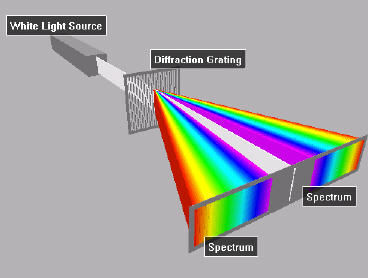
\includegraphics[width=0.9\textwidth]{M48}
\caption{Réseau de fentes}
\label{f12}
\end{marginfigure}

Un réseau de fentes (fig \ref{f12}) est un dispositif optique composé d'une série de fentes parallèles espacées de manière régulière.

\subsection{Analyse mathématique}

Comme illustré sur les figures \ref{d10}, on considère un réseau de $N$ fentes de largeur finie $a$ et de période $d$. Pour rappel, le principe de Huygens énonce que chaque fente se comporte comme la source d'une infinité d'ondelettes. On souhaite donc calculer l'intensité de l'onde résultante en un point $P$ en additionnant les ondes arrivant en P (avec le déphasage propre à chaque ondelette).

\begin{figure}[h]
\centering
\subfloat[]{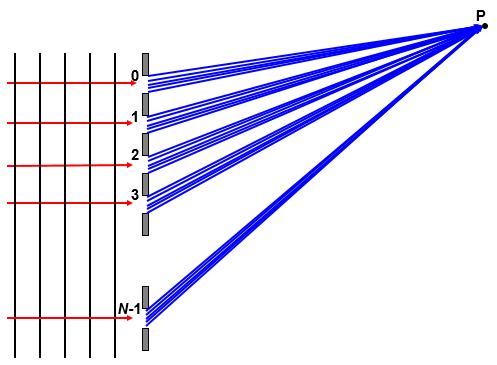
\includegraphics[width=5cm]{M41}}
        \quad
\subfloat[]{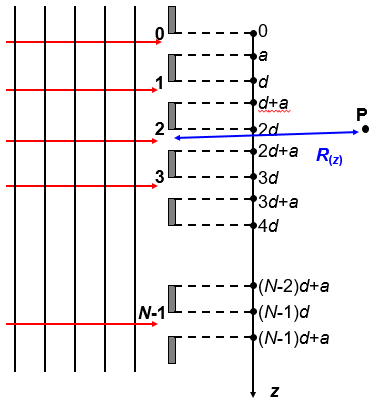
\includegraphics[width=4cm]{M42}}
\caption{Réseau de fentes}
        \label{d10}
\end{figure}

\noindent En notation complexe, le champ généré par une ondelette (source infinitésimale) en $P$ vaut
$$
 \overset\rightarrow{dE}(P)=\frac{A}{R(z)}\frac{dz}{a}\exp\big(j(kR(z)-\omega t)\big)\overset\rightarrow{\mbox{l}_y}
$$
où $\overset\rightarrow{\mbox{l}_y}$ est un vecteur unitaire perpendiculaire au plan, $A$ est l'amplitude de l'onde plane incidente, $k$ est le nombre d'onde et $R(z)$ est la distance entre la source de l'ondelette et $P$. \\
Au delà de la fente, l'amplitude décroit en $1/R$ puisque l'onde est sphérique. Le facteur $dz/a$ normalise l'amplitude pour que l'intensité dans le cas idéalisé sans diffraction (une source par fente) soit identique à la somme des intensités des sources dans une même fente:
$$
 \int_0^a\frac{A}{aR(z)}\exp\big(j(kR-\omega t)\big)dz\:\overset\rightarrow{\mbox{l}_y}=\frac{A}{R(z)}\exp\big(j(kR-\omega t)\big)\overset\rightarrow{\mbox{l}_y}=\overset\rightarrow{E_{ideal}}(P)
$$
si $R$ est le même pour chaque source.\\

\begin{marginfigure}[0cm]
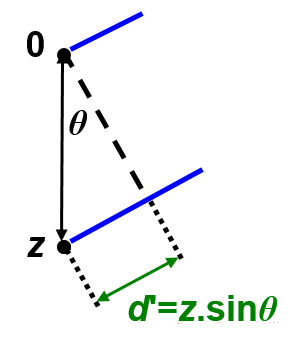
\includegraphics[width=0.9\textwidth]{M43}
\caption{Différence de chemin}
\label{f14}
\end{marginfigure}

\noindent Le champ résultant en $P$ se calcule en sommant les sources dans les $N$ fentes:
$$
  \overset\rightarrow{E(P)}=\sum_{n=0}^{N-1}\int_{nd}^{nd+a}\frac{A}{aR(z)}\exp\big(j(kR(z)-\omega t)\big)dz\:\overset\rightarrow{\mbox{l}_y}.
$$
Par l'approximation de Fraunhofer, $P$ est à l'infini et tous les rayons sont parallèles. En utilisant la figure \ref{f14}, on déduit que la direction des rayons est donnée par l'angle $\theta$ et 
$R(z)=R(z=0)+z\sin \theta$. En considérant\footnote{simplification explicitée dans le chapitre sur les interférences} $\frac{1}{R(z)}\simeq\frac{1}{R(z=0)}$,
le champ s'écrit
\begin{align*}
\overset\rightarrow{E}(P) & = \sum_{n=0}^{N-1}\int_{nd}^{nd+a}\frac{A}{aR_0}\exp\big(j(k(R_0+z\sin \theta)-\omega t)\big)dz\:\overset\rightarrow{\mbox{l}_y}\\
 &= \frac{A}{aR_0}\exp\big(j(kR_0-\omega t)\big)\sum_{n=0}^{N-1}\int_{nd}^{nd+a}\exp\big(jkz\sin \theta\big)dz\:\overset\rightarrow{\mbox{l}_y}.
\end{align*}
On peut effectuer l'intégrale et obtenir
\begin{align*}
\int_{nd}^{nd+a}\exp\big(jkz\sin \theta\big)dz & =\frac{1}{jk\sin\theta}\Big[\exp\big(jkz\sin \theta\big)\Big]_{nd}^{nd+a}\\
&=\frac{1}{jk\sin\theta}\bigg(\exp\big(jk(nd+a)\sin \theta\big)-\exp\big(jknd\sin \theta\big) \bigg)\\
&=\frac{\exp\big(jka\sin \theta\big)-1 }{jk\sin\theta}\exp\big(jknd\sin \theta\big).
\end{align*}
En utilisant la relation
$$\sum\limits_{p=0}^{N-1} x^p=\frac{1-x^N}{1-x}, $$
on transforme la somme en
\begin{align*}
\sum_{n=0}^{N-1}\exp\big(jknd\sin \theta\big)&=\frac{1-\exp\big(jkNd\sin \theta\big)}{1-\exp\big(jkd\sin \theta\big)}
\end{align*}
pour obtenir la formulation finale du champ résultant $\overset\rightarrow{E}(P)$:
$$
  \overset\rightarrow{E(P)}=\frac{A}{aR_0}\exp\big(j(kR_0-\omega t)\big)\frac{\exp\big(jka\sin \theta\big)-1 }{jk\sin\theta}\:\frac{1-\exp\big(jkNd\sin \theta\big)}{1-\exp\big(jkd\sin \theta\big)}  \:\overset\rightarrow{\mbox{l}_y}.
$$
On calcule ensuite l'intensité du champ en $P$: $I(P)=\frac{\epsilon c}{2}\overset\rightarrow{E}(P).\overset\rightarrow{E^*}(P)$. $\overset\rightarrow{E}(P)$ est un produit de 4 termes dont on peut analyser séparément l'intensité:
\begin{enumerate}
    \item $(A/aR_0)^2$
    
    \item $\exp\big(j(kR_0-\omega t)\big)\exp\big(-j(kR_0-\omega t)\big)=1$
    
    \item 
    \begin{align*}
\frac{\exp\big(jka\sin \theta\big)-1 }{jk\sin\theta}\frac{\exp\big(-jka\sin \theta\big)-1 }{-jk\sin\theta}&=\frac{2-\Big(\exp\big(jka\sin \theta\big)+\exp\big(-jka\sin \theta\big)\Big)}{(k\sin\theta)^2}\\
&=\frac{2\Big(1-\cos\big(ka\sin \theta\big)\Big)}{(k\sin\theta)^2}\\
&=\frac{4\sin^2\big(\frac{ka\sin \theta}{2}\big)}{(k\sin\theta)^2}
\end{align*}
    
    \item
    \begin{align*}
\frac{1-\exp\big(jkNd\sin \theta\big)}{1-\exp\big(jkd\sin \theta\big)}\frac{1-\exp\big(-jkNd\sin \theta\big)}{1-\exp\big(-jkd\sin \theta\big)}
&=\frac{2-\Big(\exp\big(jkNd\sin \theta\big)+\exp\big(-jkNd\sin \theta\big)\Big)}{2-\Big(\exp\big(jkd\sin \theta\big)+\exp\big(-jkd\sin \theta\big)\Big)}\\
&=\frac{1-\cos(kNd\sin \theta)}{1-\cos(kd\sin \theta)}\\
&=\frac{\sin^2\big(\frac{kNd\sin \theta}{2}\big)}{\sin^2\big(\frac{kd\sin \theta}{2}\big)}
\end{align*}
    
\end{enumerate}
L'intensité s'exprime finalement sous la forme
\begin{align*}
I(P)&=\frac{\epsilon c}{2}\frac{A^2}{a^2R_0^2}\frac{4\sin^2\big(\frac{ka\sin \theta}{2}\big)}{(k\sin\theta)^2}\frac{\sin^2\big(\frac{kNd\sin \theta}{2}\big)}{\sin^2\big(\frac{kd\sin \theta}{2}\big)}\\
&=I_0
\underbrace{\frac{\sin^2\big(\frac{\pi a\sin \theta}{\lambda}\big)}{\big(\frac{\pi a\sin\theta}{\lambda}\big)^2}}_{%
     \footnotesize\begin{tabular}{c}Diffraction\\par une fente\end{tabular}}
\underbrace{\frac{\sin^2\big(\frac{\pi Nd\sin \theta}{\lambda}\big)}{\sin^2\big(\frac{\pi d\sin \theta}{\lambda}\big)}}_{%
     \footnotesize\begin{tabular}{c}Réseau de\\fentes idéales\end{tabular}}
\end{align*}
Tenir compte de l'effet de diffraction pour un réseau de fentes revient donc simplement à multiplier les intensité normalisées ($I/I_0$) liées à la diffraction à travers une fente simple et liées à un réseau de fentes idéales.

\subsection{Interprétation de l'intensité}
Dans la direction normale à la fente, le premier quotient vaut
\begin{align*}
\frac{\sin^2\big(\frac{\pi a\sin \theta}{\lambda}\big)}{\big(\frac{\pi a\sin\theta}{\lambda}\big)^2}&\overset{\frac{0}{0}}{=}\frac{2\sin\big(\frac{\pi a\sin \theta}{\lambda}\big)\cos\big(\frac{\pi a\sin \theta}{\lambda}\big)\frac{\pi a\cos \theta}{\lambda}}{2\big(\frac{\pi a\sin\theta}{\lambda}\big)\big(\frac{\pi a\cos\theta}{\lambda}\big)}\\
&=\frac{\sin\big(2\frac{\pi a\sin \theta}{\lambda}\big)}{\frac{\pi a\sin \theta}{\lambda}}\\
&\overset{\frac{0}{0}}{=}\frac{\cos\big(2\frac{\pi a\sin \theta}{\lambda}\big)(\frac{\pi a\cos \theta}{\lambda})}{\frac{\pi a\cos \theta}{\lambda}}\\
&=1.
\end{align*}
Le second quotient vaut $N^2$ car la relation
$$
\lim_{\theta \rightarrow 0}\frac{\sin^2\big(\frac{\pi Nd\sin \theta}{\lambda}\big)}{\sin^2\big(\frac{\pi d\sin \theta}{\lambda}\big)}=N^2
$$
a été démontrée dans le chapitre précédent.
L'intensité vaut donc
$$
    I(P)=N^2I_0
$$
dans la direction normale.\\

\noindent Le premier quotient exprime l'intensité diffractée par une seule fente de largeur $a$ alors que le second donne l'expression de l'intensité diffractée par un réseau de $N$ fentes idéales de période $d$ (et de largeur nulle). La figure \ref{d11} illustre graphiquement l'intensité (en vert) résultant du produit des deux termes (en rouge et bleu).

\begin{figure}[h!]
    \centering
    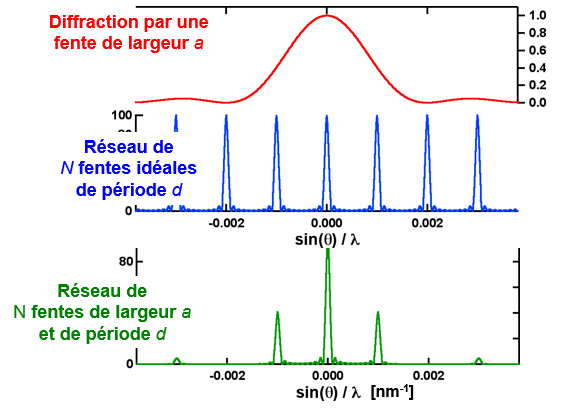
\includegraphics[scale=0.6]{M44}
    \caption{Graphes (rouge, bleu, vert) de l'intensité en fonction de la direction de propagation d'une onde traversant une réseau de fentes pour $N=10, a=500$ nm et $d=1000$ nm}
    \label{d11}
\end{figure}

\noindent Les pics et petits zéros auxiliaires sont dûs au second quotient. Les \textbf{pics} apparaissent quand le numérateur et le dénominateur sont nuls pour un même angle $\theta$, c'est-à-dire lorsque\footnote{une autre condition due à l'effet de diffraction doit être prise en compte, elle est établie à la page suivante}
$$
    \frac{\pi d\sin \theta}{\lambda}=m\pi\Rightarrow d\sin \theta=m\lambda \qquad(\forall m\in  \mathbb{Z}).
$$
On appelle $m$, l'ordre du pic.

Les \textbf{petits zéros auxiliaires} surviennent quand le numérateur s'annule et le dénominateur est non nul:
$$
    \frac{N\pi d\sin \theta}{\lambda}=n\pi\Rightarrow d\sin \theta=\frac{n}{N}\lambda \qquad(\forall n\in  \mathbb{Z} \mbox{ et si } \frac{n}{N}\notin  \mathbb{Z}).
$$
La condition $\frac{n}{N}\notin  \mathbb{Z}$ implique qu'il ne s'agit pas d'un pic.

Sur la figure \ref{d12}, les conditions sont:
\begin{itemize}
    \item $ \sin \theta/\lambda=m/d=m/1000\:[nm^{-1}]$ pour un pic
    \item $\sin \theta/\lambda=n/(Nd)=n/10^4\:[nm^{-1}]$ si $n/10\notin  \mathbb{Z}$ pour un petit zéro auxiliaire
\end{itemize}

\begin{figure}[h!]
    \centering
    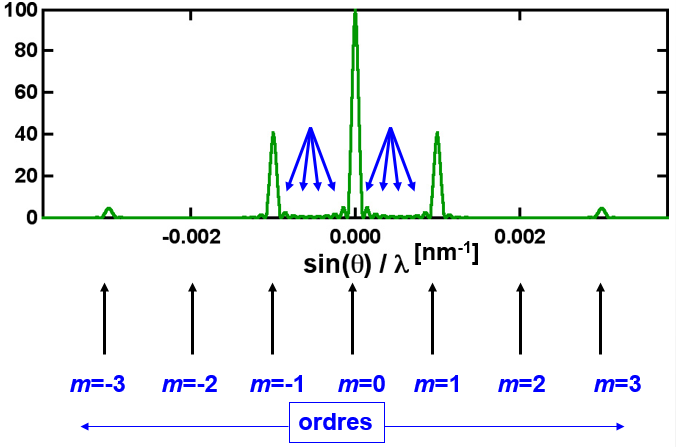
\includegraphics[scale=0.4]{M45}
    \caption{Petits zéros auxiliaires et pics d'intensité}
    \label{d12}
\end{figure}

\noindent Le premier quotient de l'expression de l'intensité fournit l'enveloppe du graphe de l'intensité (fig \ref{d13}), elle passe par tous les sommets locaux du graphe vert. Lorsque celle-ci s'annule, l'intensité est également nulle quelque soit la valeur du second quotient. Cette enveloppe vaut $0$ quand le numérateur est nul:
$$
    \frac{\pi a\sin \theta}{\lambda}=p\pi\Rightarrow a\sin \theta=p\lambda \qquad(\forall p\in  \mathbb{Z}_0).
$$
Quand la direction $\theta$ est un pic pour le second quotient mais que le premier quotient s'annule, le pic est \textit{éteint}. Cet effet apparaît quand les conditions d'un pic et d'un zéro de l'enveloppe sont vérifiées pour une même direction $\theta$:
\[
\left\{
\begin{array}{ccc}
 d\sin \theta&=&m\lambda \\
 a\sin \theta&=&p\lambda               
\end{array}
\right.
\Longrightarrow
\frac{d}{a}=\frac{m}{p}\in \mathbb{Q}.
\]
Les directions $\theta$ qui produisent un pic éteint s'obtiennent en transformant la condition d'un zéro d'enveloppe pour la comparer avec la condition d'un pic:
$$
    \frac{\sin\theta}{\lambda}=\frac{p}{a}=\frac{pd/a}{d}\qquad(\forall p\in  \mathbb{Z}_0),
$$
elle correspond au pic d'intensité si $pd/a$ est entier. Dans le cas des graphiques présentés dans cette section, $pd/a=2p$ est toujours un nombre entier et les directions éteintes sont 
$$
    \frac{\sin\theta}{\lambda}=\frac{2p}{d}=0,002p\:[nm^{-1}] \qquad(\forall p\in  \mathbb{Z}).
$$
On dit alors que les ordres pairs sont éteints puisque les directions pour lesquelles l'ordre $m$ est pair ont une intensité nulle.\\

\begin{figure}[h!]
    \centering
    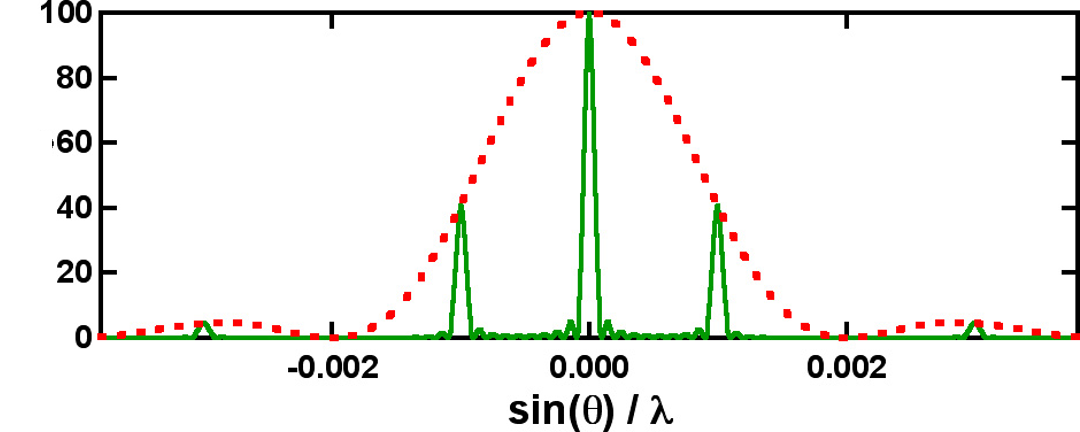
\includegraphics[scale=0.4]{M46}
    \caption{Enveloppe donnée par la courbe de diffraction d'une fente}
    \label{d13}
\end{figure}

\noindent On souhaite maintenant calculer la largeur du premier lobe, c'est-à-dire la distance entre les 2 petits zéros auxiliaires les plus proches du centre de la figure. Le premier zéro de droite est donné par
$$
    \frac{\sin\theta}{\lambda}=\frac{1}{Nd}\Longrightarrow \theta=\arcsin\Big(\frac{\lambda}{Nd}\Big).
$$
Par symétrie, la variations angulaire délimitée par le premier lobe vaut
$$
    \Delta\theta=2\arcsin\Big(\frac{\lambda}{Nd}\Big) \Longleftrightarrow \Delta\Big(\frac{\sin\theta}{\lambda}\Big)=\frac{2}{Nd}.
$$
La figure \ref{d14} montre bien que la largeur des lobes\footnote{exprimée en fonction de $\sin\theta/\lambda$ et non en fonction de $\theta$} est inversement proportionnelle au nombre de fentes.

\begin{figure}[h!]
    \centering
    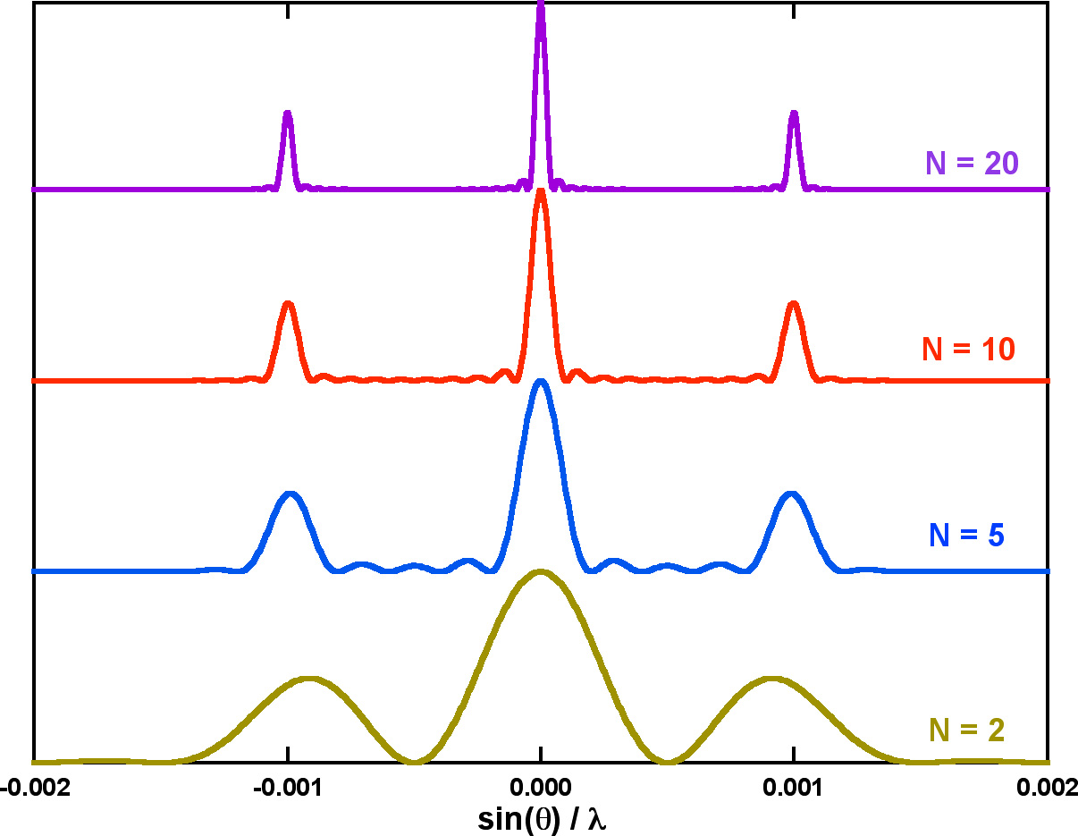
\includegraphics[scale=0.4]{M47}
    \caption{Graphe analysant la largeur des lobes pour différentes valeurs de $N$ (avec $a=500$ nm et $d=1000$ nm)}
    \label{d14}
\end{figure}

\subsection{Séparation chromatique par un réseau de diffraction}

La \textit{spectroscopie} est l'étude expérimentale du spectre d'un phénomène physique\footnote{par exemple le rayonnement émis par une étoile ou un matériau.}, c'est-à-dire de sa décomposition sur une échelle d'énergie, et plus particulièrement dans ce chapitre selon la longueur d'onde. C'est l'analogue de la transformée de Fourier qui analyse le contenu fréquentiel d'un signal.\\

\begin{figure}[h!]
    \centering
    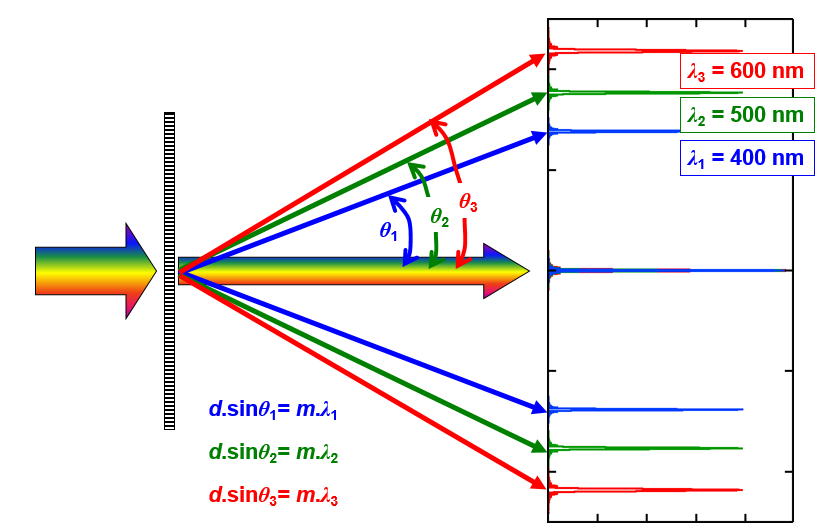
\includegraphics[scale=0.4]{M51}
    \caption{Schéma d'un spectroscope et de la figure de diffraction d'une lumière blanche traversant un réseau de fentes}
    \label{d16}
\end{figure}

\noindent Pour décomposer une onde selon ses longueurs d'ondes, on fait passer cette onde à travers un réseau de fentes, l'onde transmise est ensuite analysée sur une plaque noire parallèle placée derrière le réseau de fente. Comme illustré sur la figure \ref{d16}, la position des pics secondaires diffère selon la longueur d'onde. On peut donc décomposer l'onde incidente selon la direction $\theta$. Par exemple, la couleur visible (violet) la plus proche du centre fait un angle tel que $\sin\theta_v=\lambda_v/d=380\:nm/d$ et la couleur visible (rouge) la plus éloignée du centre fait un angle tel que $\sin\theta_r=\lambda_r/d=780\:nm/d$. La figure \ref{d15} illustre la partie gauche de la figure de diffraction, allant du rouge vers le bleu.\\

\noindent Un objet opaque recevant de la lumière réfléchit celle-ci pour certaines longueurs d'onde particulières (c'est ce qui explique la couleur des objets). La photo supérieure de la figure \ref{d15} est le spectre d'un corps chaud, par exemple une étoile. Ce corps est perçu blanc par l'oeil humain car il renvoie toute la lumière (son spectre est composé de toutes les couleurs\footnote{c'est-à-dire toutes les longueurs d'onde entre $380$ et $780$ nm}).

\noindent Le spectre du centre est celui d'un gaz élémentaire chaud, il a des raies d'émissions caractéristiques de sa composition atomique. Chaque atome excité émet des ondes (énergie) de manière discrète (par quanta) dont les énergies sont données par la mécanique quantique. Par exemple, une lampe à néon, qui semble envoyer une lumière blanche comme celle du soleil, n'émet que des ondes pour quelques longueurs d'onde précises donnée par les caractéristiques de l'atome du Néon.

\noindent Le spectre inférieur de la figure \ref{d15} est celui d'un corps chaud dont la radiation passe à travers un gaz plus froid dont le spectre est sur la photo du centre. Ce gaz absorbe toutes les ondes dont la longueur d'onde se trouve dans une partie visible de son spectre. Ainsi, le corps chaud, dont le spectre est initialement celui de la photo supérieure, aura quelques longueurs d'onde absorbées par le gaz. Il n'en restera donc que le spectre complémentaire.\\

\noindent Cette technique est utilisée par exemple en astronomie. Quand la lumière venant du soleil traverse son atmosphère, certaines longueurs d'onde sont sélectivement absorbées. Des expériences en laboratoire ont montré que les atomes et ions absorbent des longueurs d'ondes propres à chaque élément. En comparant le spectre de la lumière solaire avec ces résultats en laboratoire, les astronomes en déduisent la composition chimique de l'atmosphère autour du soleil. La même technique est utilisée pour faire des essais chimiques sur les galaxies lointaines.

\begin{figure}[h!]
    \centering
    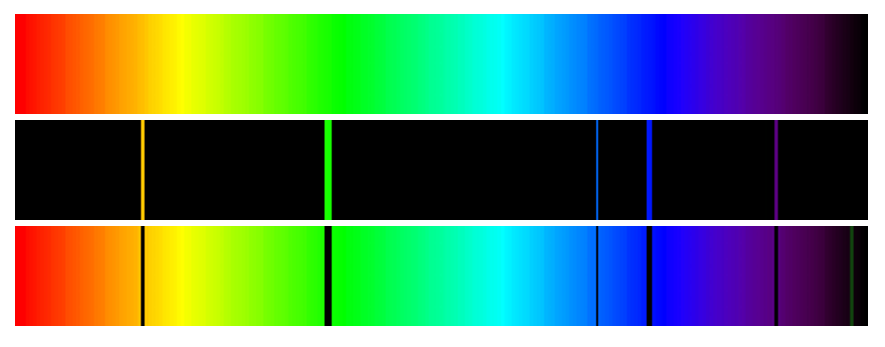
\includegraphics[scale=0.35]{M49}
    \caption{Spectres de trois corps chauds}
    \label{d15}
\end{figure}

\noindent En astronomie, il faut aussi tenir compte de l'\textit{effet Doppler}. La longueur d'onde du rayonnement reçu est plus grande lorsque la source s'éloigne, et plus courte lorsque la source se rapproche.
Cet effet explique en particulier le décalage vers le rouge\sidenote[][-2cm]{l'augmentation de la longueur d'onde la rapproche de celle du rouge, qui est la plus grande longueur d'onde visible} observé dans le spectre de la lumière d'un astre qui s'éloigne à l'observateur.\\

\begin{marginfigure}[-1cm]
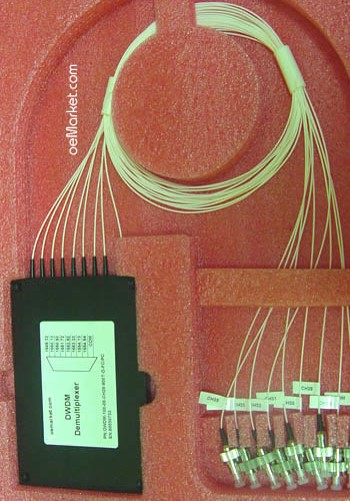
\includegraphics[width=0.7\textwidth]{M50}
\caption{Multiplexage}
\label{f15}
\end{marginfigure}

\noindent Le \textit{multiplexage en longueur d'onde}, montré sur la figure \ref{f15}, est une technique utilisée en communication optique qui permet d'augmenter le débit sur une fibre optique en faisant circuler plusieurs signaux de longueurs d'onde différentes sur une seule fibre, en les mélangeant à l'entrée à l'aide d'un multiplexeur et en les séparant à la sortie au moyen d'un démultiplexeur. Les équipements de démultiplexage utilisent généralement des réseaux de diffraction. Ils agissent comme des filtres en sélectionnant le signal dans une zone de longueur d'onde donnée.\\

\noindent Ce procédé n'est pas restreint aux ondes du spectre visible, il est aussi valable en projetant des rayons infrarouges par exemple. La \textit{spectroscopie d'infra-rouge} permet de déterminer la présence de groupements fonctionnels dans les molécules organiques, et les structures dans certaines molécules simples. Dans les molécules, les liaisons vibrent à une fréquence bien déterminée qui dépend des atomes de la liaison. Pour une fréquence donnée, ces liaisons rentrent en résonance: l'énergie apportée est alors consommée, les molécules absorbent et la transmission diminue. Le spectre d'absorption d'un matériau permet de déterminer avec précision sa composition moléculaire.

\subsection{Pouvoir de résolution chromatique}

Quand une onde n'est pas monochromatique (une seule longueur d'onde), le graphe de l'intensité ne caractérise pas avec une précision totale les longueurs d'onde qui composent l'onde incidente. En effet, si l'on considère deux longueurs d'onde assez proches, par exemple le bleu et violet, le graphe de l'onde mixte est donné par la somme des graphes d'une onde composée de bleu et d'une autre composée de violet. On remarque sur la figure \ref{d17} que l'intensité résultante ne possède qu'un seul pic pour une longueur d'onde entre celle du bleu et du violet. Par contre, l'assemblage bleu/rose produit un graphe avec deux pics en $\lambda_{rose}$ et en $\lambda_{bleu}$. Il est donc possible de déterminer ces deux longueurs d'onde à partir du graphe de la somme des intensités.\\

\noindent Par définition, deux raies sont résolues si le maximum de la première raie est en dehors du premier lobe de le seconde raie. On en déduit donc par la figure \ref{d17} que le bleu/violet n'est pas résolu alors que le bleu/rose est résolu.


\begin{figure}[h!]
    \centering
    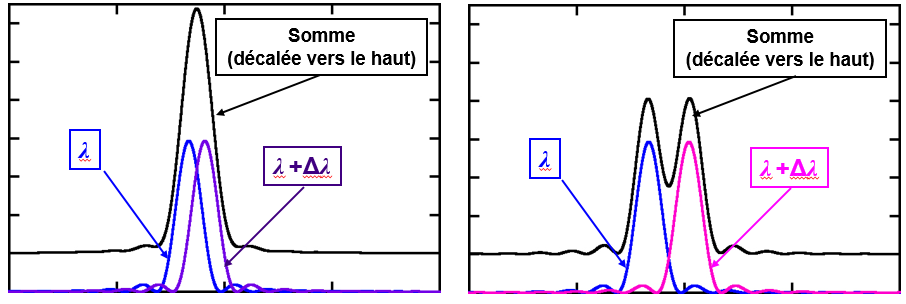
\includegraphics[scale=0.4]{M52}
    \caption{Résolution chromatique entre deux couleurs: bleu/violet et bleu/rose}
    \label{d17}
\end{figure}

\noindent La condition limite de résolution entre 2 longueurs d'onde est appelée le \textit{pouvoir de résolution} d'un réseau de fentes et vaut
$$
    \frac{\lambda}{\Delta\lambda},
$$
 il indique la valeur du décalage $\Delta\lambda$ maximum que l'on peut ajouter à la longueur d'onde initiale tout en gardant la résolution chromatique. La valeur maximale s'obtient quand le maximum de la première raie (1) correspond au premier zéro de la seconde raie (2):
\[
\left\{
\begin{array}{ccc}
 (1)\:d\sin \theta&=&m\lambda\\
 (2)\:d\sin \theta&=&(m\pm\frac{1}{N})(\lambda+\Delta\lambda)
\end{array}
\right.
\Longrightarrow
\frac{\lambda}{\Delta\lambda}=mN\pm1\simeq mN.
\]
Le $\pm$ tient compte du décalage $\Delta\lambda$ vers la gauche ou vers la droite par rapport à la longueur d'onde initiale. Il n'est cependant pas important car on peut supprimer $\pm1$ ($mN>>1$).
On perd donc la résolution en ajoutant moins que $\lambda/(mN)$ à la longueur d'onde initiale.


\subsection{Réseaux bidimensionnels et tridimensionnels (à titre informatif)}

Les rayons X ont été découverts par Rontgen en 1895, mais des expériences antécédentes annonçaient déjà la présence d'ondes électromagnétiques avec des longueurs d'onde de l'ordre de $10^{-10}$ m. Max von Laue a proposé en 1912 qu'un cristal, dont la distance interatomique vaut environ $10^{-10}$ m, pourrait servir de réseau de diffraction 3D pour les rayons X.
La théorie de la \textit{diffraction sur un cristal} modélise l'interaction rayonnement-matière dans le cas où la matière est organisée de manière ordonnée. Le phénomène à la base de la diffraction par un cristal est la diffusion du rayonnement par les atomes. 
Lorsqu'un faisceau est orienté vers une structure cristalline, une image est engendrée par la combinaison des ondes sphériques émanant de chaque atome excité par l'onde incidente. La figure \ref{d18} illustre le processus sur un cristal de diamant excité par des rayons X dont la longueur d'onde vaut environ $0,154$ nm. Remonter de l'image des interférences à la structure intime de la matière est néanmoins assez complexe et toujours en développement, surtout pour un réseau tridimensionnel.
Actuellement, ce procédé est beaucoup utilisé en science des matériaux (nano-objets), ou en biologie pour analyser la structure de protéines, virus, complexes,...

\begin{figure}[h!]
    \centering
    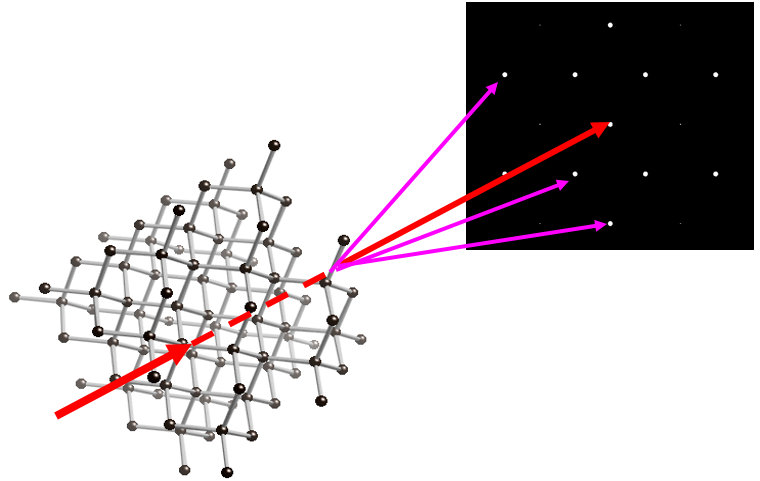
\includegraphics[scale=0.4]{M53}
    \caption{Projection de rayons X sur un cristal de carbone diamant
}
    \label{d18}
\end{figure}

\begin{marginfigure}
	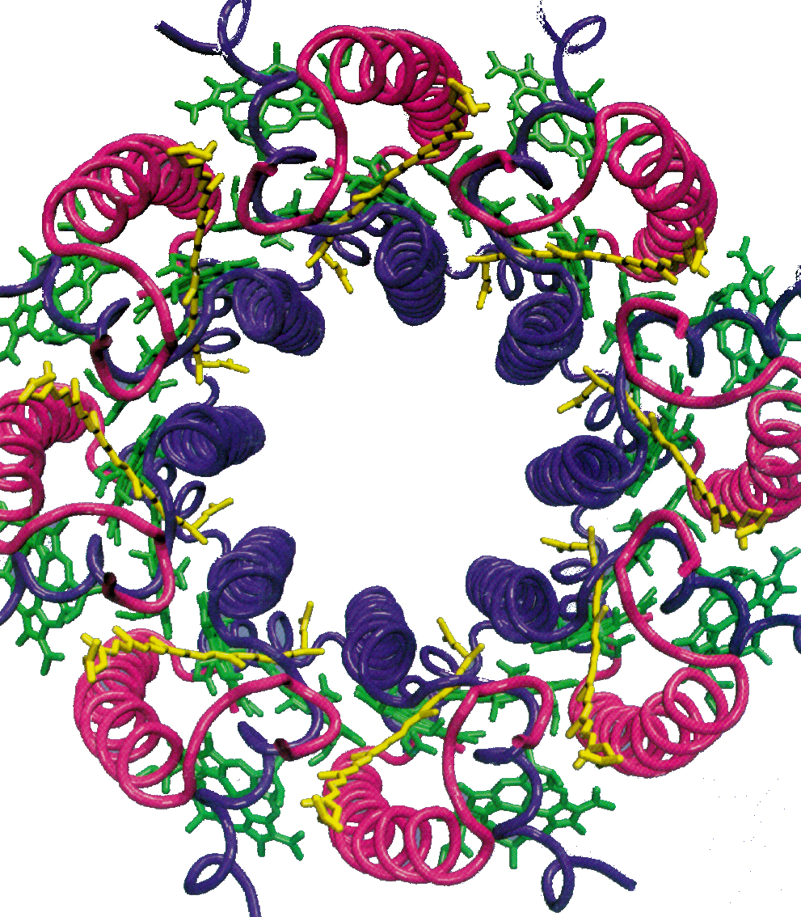
\includegraphics[scale=0.3]{M54}
	\caption{centre de capture de la lumière d'une bactérie photo-synthétique: \textit{LH II Rs. molisch}
	}
	\label{d19}
\end{marginfigure}

\noindent La reproduction sur la figure \ref{d19} est un exemple du type de structure qui peut être résolue à l'heure actuelle. Les couleurs représentent le même type de molécule: des bactério-chlorophylles en vert, des caroténoïdes en jaune, des Apo-protéines (hélice $\alpha$) en bleu, des Apo-protéines (hélice $\beta$) en rose.




 